Since the purpose is to make a function of structural features to desired 
properties, in this section, we will discuss about which features should be 
chosen as variables for the functions. The variables’ roles are not only to 
form relationships to desired properties, but also to distinguish different 
data points. To avoid unnecessary complexity, the variables (or structural 
features) should be independent.

In alcohol, it is already understood that the number of OH groups 
significantly affect the ability of heat transfer while the position of the OH 
group also change the properties values \cite{manjunatha_investigation_2017}. However, there 
might be also other potential structural features that are left uninvestigated. 
Since we only care about the impact of the structural features on the 
thermophysical properties, we will select all the features that define an 
alcohol molecular structure.
\newpage
\begin{figure}[h!]
    \centering
    \begin{subfigure}[b]{0.3\linewidth}
      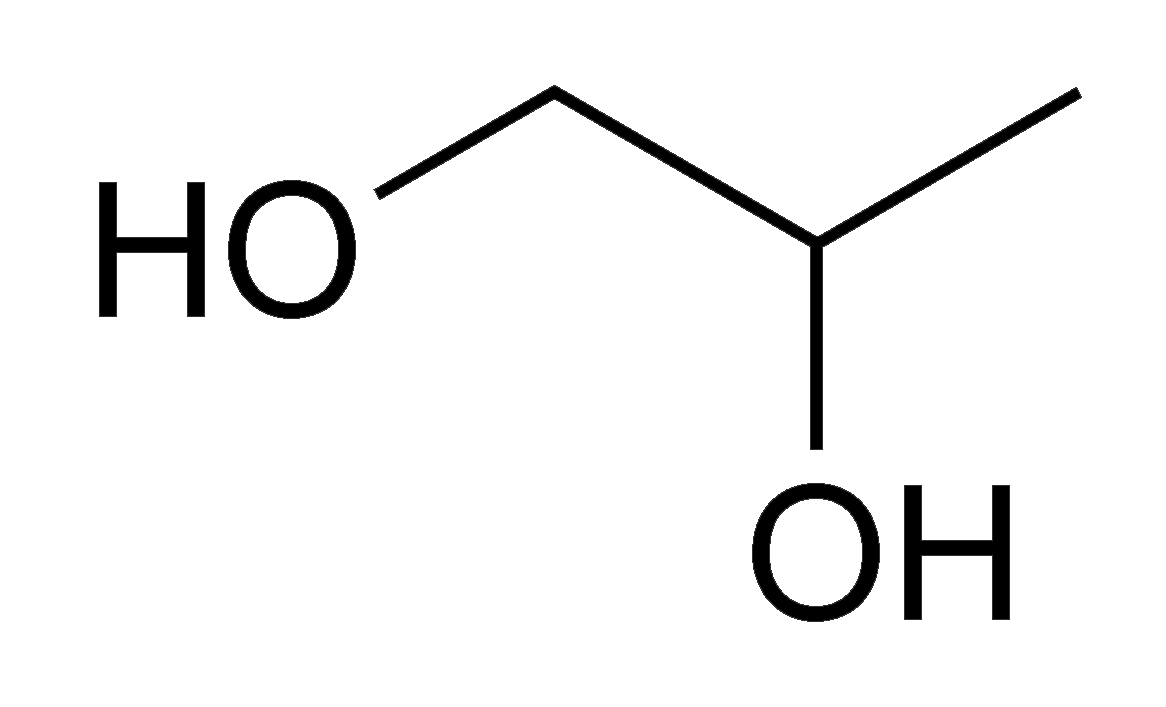
\includegraphics[width=\linewidth]{prplene.png}
       \caption{Propylene Glycol}
    \end{subfigure}
    \begin{subfigure}[b]{0.3\linewidth}
      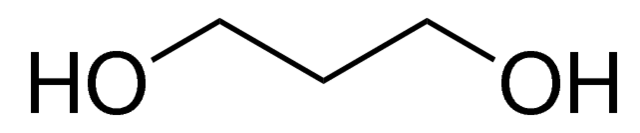
\includegraphics[width=\linewidth]{13prop.png}
      \caption{1,3-propanediol}
    \end{subfigure}
    \begin{subfigure}[b]{0.3\linewidth}
        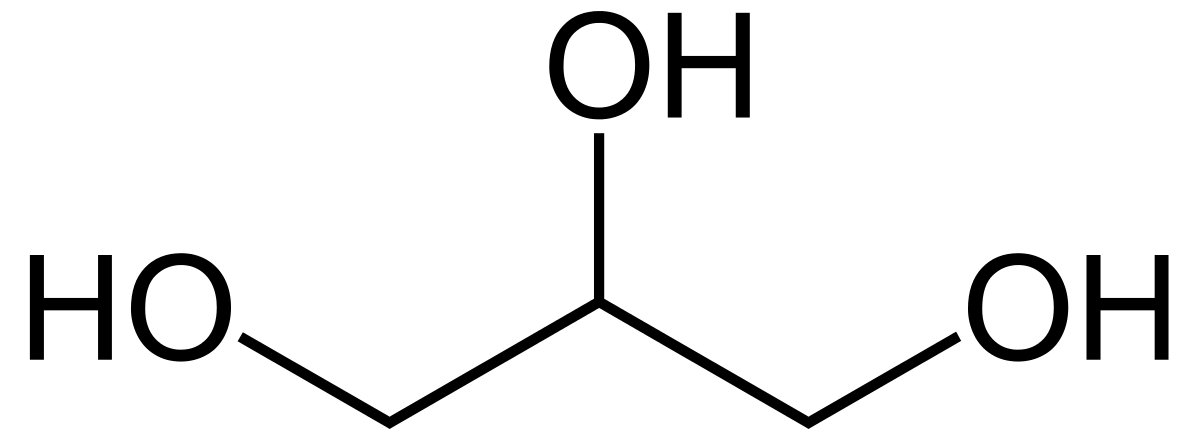
\includegraphics[width=\linewidth]{glycerol.png}
        \caption{Glycerol}
      \end{subfigure}
    \begin{subfigure}[b]{0.3\linewidth}
      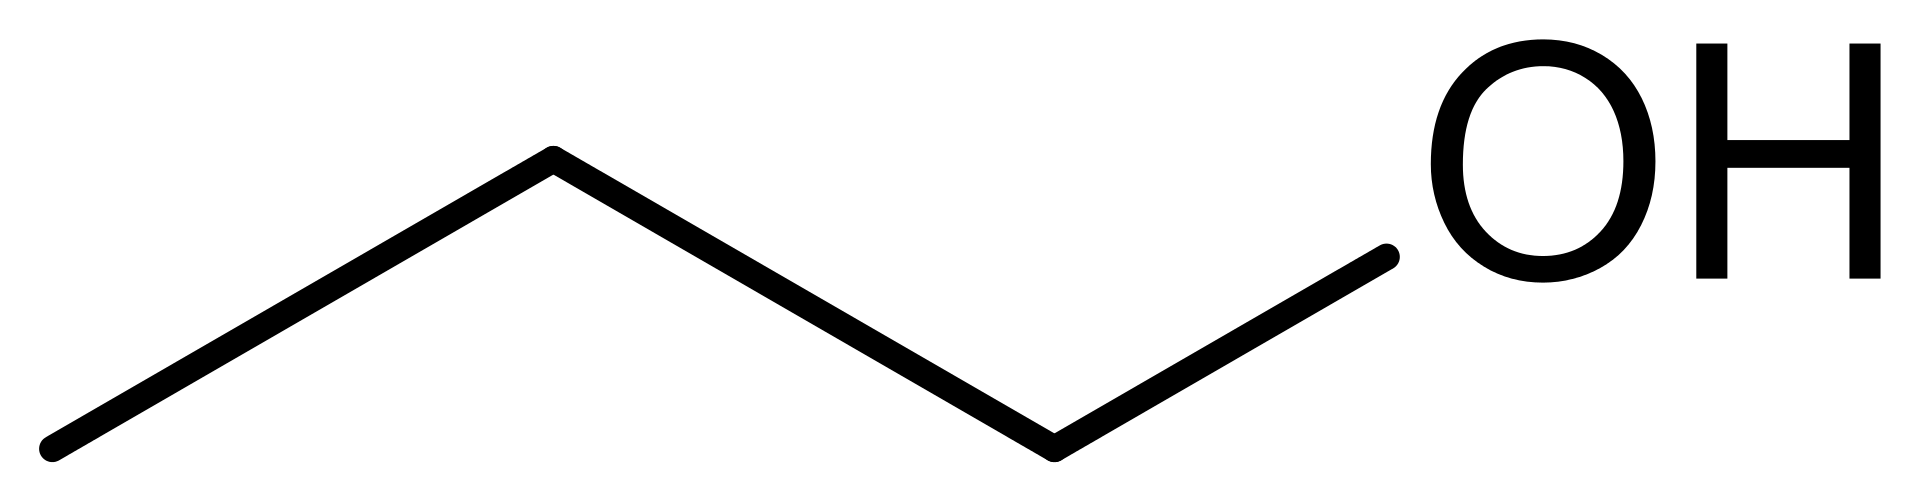
\includegraphics[width=\linewidth]{1prop.png}
      \caption{1-propanol}
    \end{subfigure}
    \begin{subfigure}[b]{0.3\linewidth}
      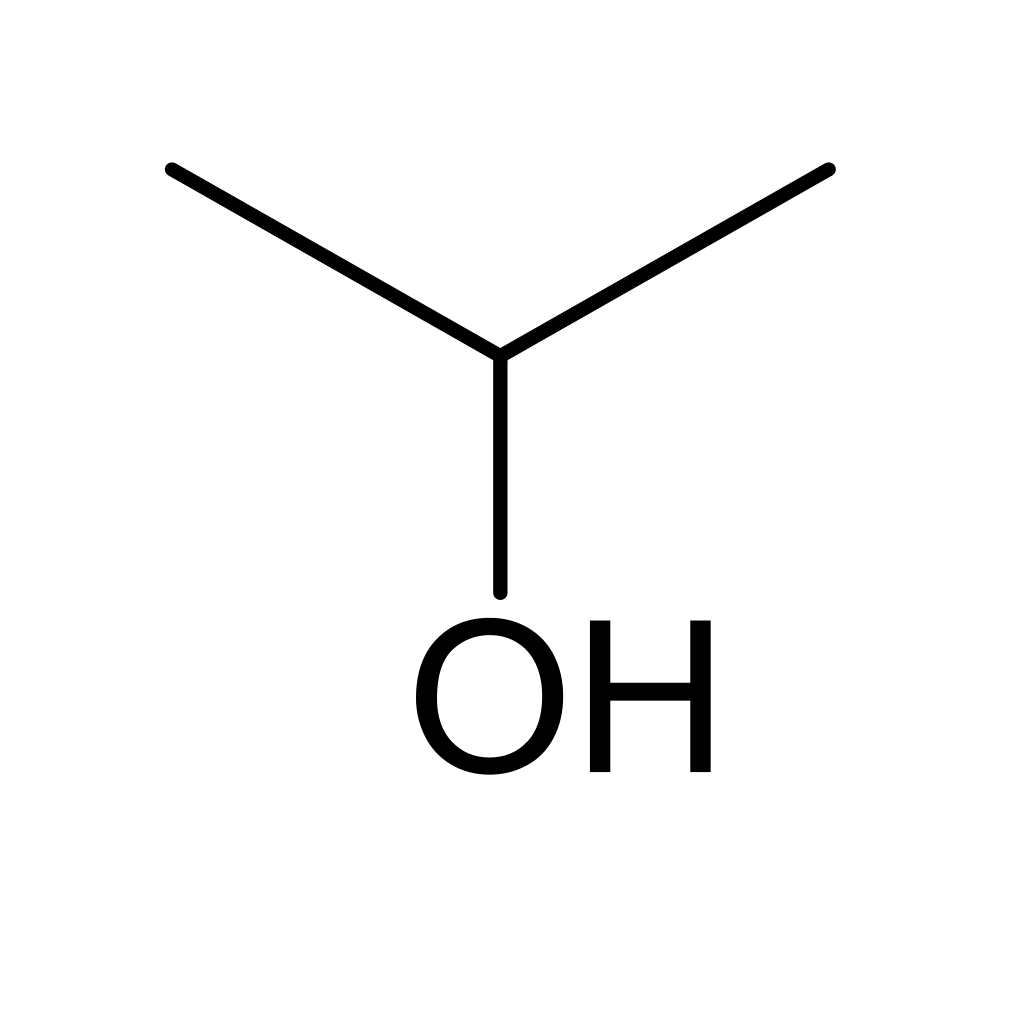
\includegraphics[width=\linewidth]{2prop.png}
      \caption{2-propanol}
    \end{subfigure}
    \begin{subfigure}[b]{0.3\linewidth}
        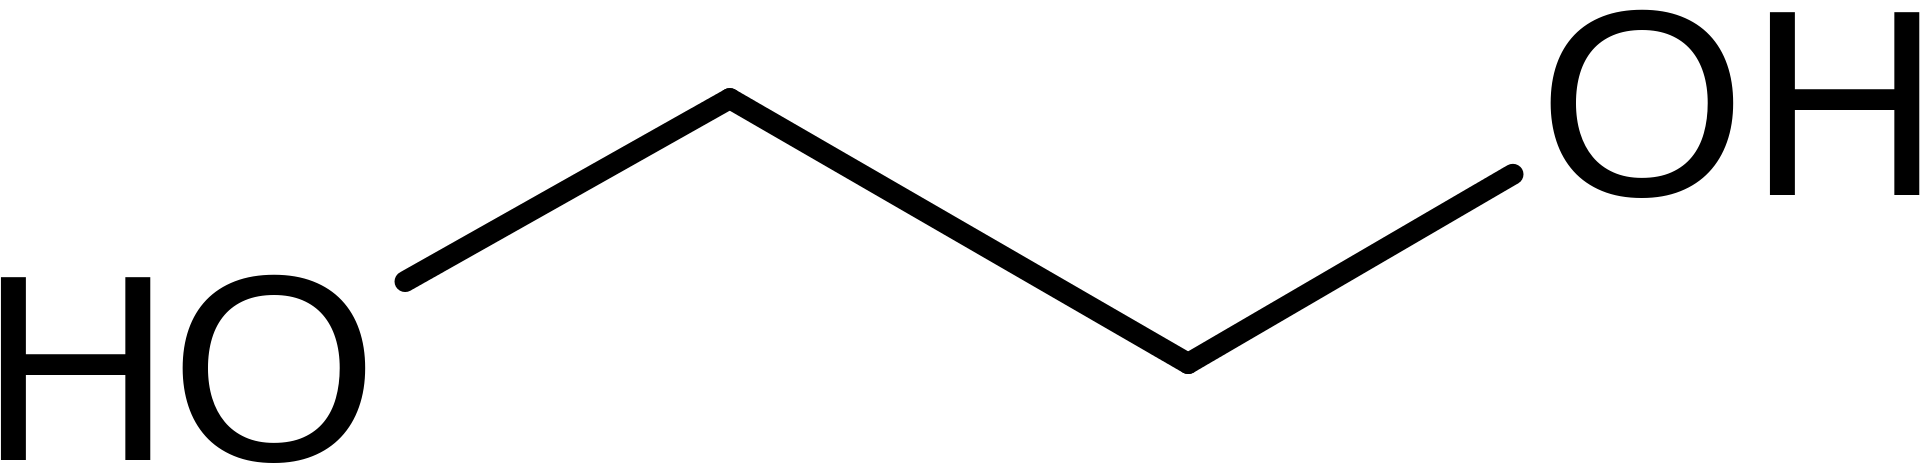
\includegraphics[width=\linewidth]{ethlne.png}
        \caption{Ethylene Glycol}
      \end{subfigure}
      \begin{subfigure}[b]{0.3\linewidth}
        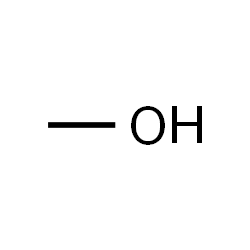
\includegraphics[width=\linewidth]{meth.png}
        \caption{Methanol}
      \end{subfigure}
      \begin{subfigure}[b]{0.3\linewidth}
        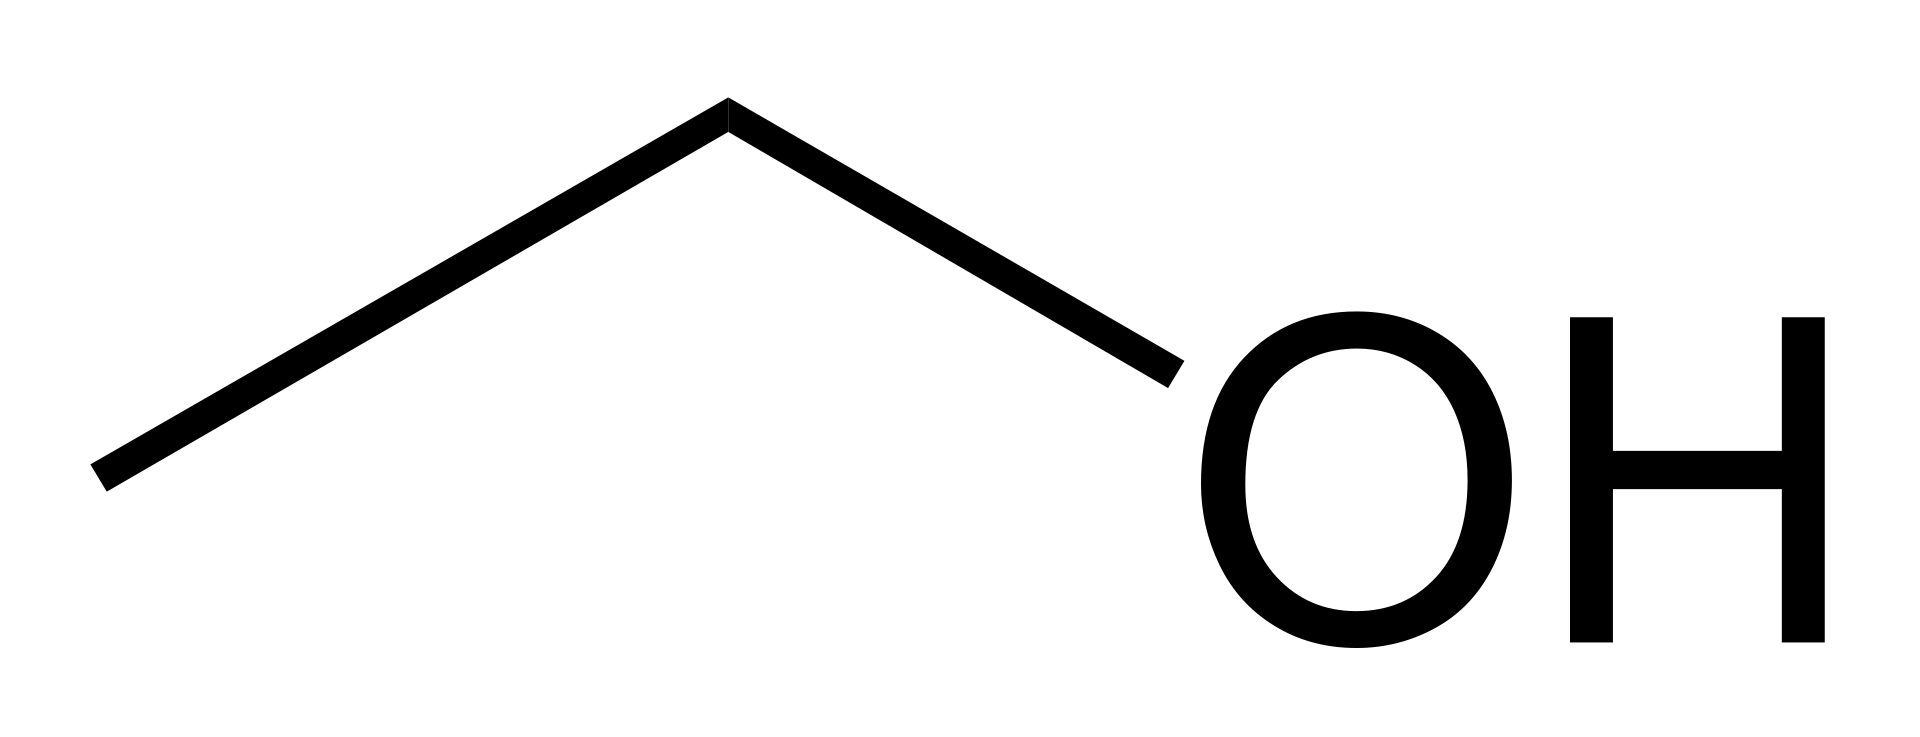
\includegraphics[width=\linewidth]{ethanol.png}
        \caption{Ethanol}
      \end{subfigure}
    \caption{ Molecular Structures of Sample Alcohol Types}
    \label{fig:mol}
\end{figure}
As we can see, there are not many significant differences and are a lot of 
similarities across the molecular structures of all the selected alcohols. 
Thus, to distinguish different alcohols, the following features (in a 
molecular structure) will be used:\\
- Number of oxygen atoms\\
- Number of carbon atoms\\
- Number of single bonds, which also represents the number of hydrogen atoms\\
- The length of the main carbon chain\\
- The position(s) of the hydroxyl group(s)\\
To differentiate between different mixtures, the following features will be used:\\
- Number of water molecules\\
- Number of alcohol molecules\\
We can also see that glycerol is the only alcohol type that possess 3 hydroxyl 
groups while propylene glycol is really close to 1,3-propanediol 
(only different in the position of the 2nd hydroxyl group). Meanwhile, 
ethanol is quite similar to methanol and 1-propanol is a structural isomer 
of 2-propanol. Interestingly, among all the above alcohol types, methanol 
is the only type that is less viscous than water.
